\documentclass[12pt]{article}
\usepackage[paper=letterpaper,margin=2cm]{geometry}
\usepackage{amsmath}
\usepackage{amssymb}
\usepackage{amsfonts}
\usepackage{newtxtext, newtxmath}
\usepackage{enumitem}
\usepackage{titling}
\usepackage{svg}
\usepackage{xcolor}
\usepackage{listings}
\usepackage{float}
\usepackage{nicefrac}
\usepackage{paracol}
\usepackage[most]{tcolorbox}
\usepackage[colorlinks=true]{hyperref}

\setlength{\droptitle}{-6em}

\definecolor{codegreen}{rgb}{0,0.6,0}
\definecolor{codegray}{rgb}{0.5,0.5,0.5}
\definecolor{codepurple}{rgb}{0.58,0,0.82}
\definecolor{backcolour}{rgb}{0.95,0.95,0.92}
\definecolor{bg}{rgb}{1,0.96,0.9}

\lstdefinestyle{mystyle}{
  commentstyle=\color{codegreen},
  keywordstyle=\color{magenta},
  numberstyle=\tiny\color{codegray},
  stringstyle=\color{codepurple},
  basicstyle=\ttfamily\footnotesize,
  breakatwhitespace=false,
  breaklines=true,
  captionpos=b,
  keepspaces=true,
  numbers=left,
  numbersep=5pt,
  showspaces=false,
  showstringspaces=false,
  showtabs=false,
  tabsize=2
}

\lstset{
  style=mystyle,
  inputencoding=utf8,
  extendedchars=true,
}


\begin{document}
\begin{enumerate}[leftmargin=\labelsep]
  \begin{tcolorbox}[enhanced jigsaw,halign=center,colback=bg,boxrule=0pt,arc=1pt]
    \item Consider the following unlabeled training data:
    \begin{table}[H]
      \centering
      \begin{tabular}{c|c|c}
              & $y_1$ & $y_2$ \\ \hline
        $x_1$ & 0     & 0     \\
        $x_2$ & 1     & 0     \\
        $x_3$ & 0     & 2     \\
        $x_4$ & 2     & 2
      \end{tabular}
    \end{table}

    Consider also the following initialization centroids:

    \begin{equation*}
      \mu_1 = \begin{bmatrix}
  80\\
  203.333\\
\end{bmatrix}, \quad \mu_2 = \begin{bmatrix}
  2\\
  1\\
\end{bmatrix}
    \end{equation*}

    \begin{enumerate}
      \item Apply $k$-means until convergence. What are the final centroids?
      \item Plot the data points and draw the clusters (with their respective centroids).
      \item Compute the silhouette score for sample $x_1$, cluster $c_1$ and for the overall solution.
      \item As the ground truth, take $x_3$ as a "negative" sample and the rest as "positive".
            Compute the error classification rate (ECR) of $k$-means here against the ground truth.
    \end{enumerate}
  \end{tcolorbox}

  For starters, it's probably worth it to write a general explanation of how $k$-means works.
  Basically, $k$-means is a clustering algorithm which, given a set of $n$ data points $\{x_1, \ldots, x_n\}$,
  tries to assign each data point to one of $k$ clusters. Each cluster is centered around
  a centroid $\mu_i$; while other clustering algorithms may create clusters of different shapes,
  $k$-means clusters are always circular/spherical. The algorithm works as follows:

  \begin{enumerate}
    \item Initialize the centroids $\mu_1, \ldots, \mu_n$.
    \item Assign each data point to the closest centroid.
    \item Recompute the centroids based on the assigned data points.
    \item Repeat steps b) and c) until convergence - that is, until the centroids don't change anymore
          (or until the change is below a certain threshold).
  \end{enumerate}

  In $k$-means solution implementations, we usually perform a series of runs with different
  centroid initializations and pick the best one (where the \textit{best} here
  is defined by a combination of metrics, which we'll discuss later). In the following
  exercises, though, we'll just use a single run. We'll also be using the Euclidean distance here,
  the most common distance metric used in this algorithm.

  For starters, let's assign each sample to the closest centroid. We can do this by computing
  the distance between each sample and each centroid, and then picking the centroid with the
  smallest distance:

  \begin{equation*}
    \left\| x_1 - \mu_1 \right\| = \left\| \begin{bmatrix}
  1 & 0 & 0 & 0\\
\end{bmatrix} - \begin{bmatrix}
  80\\
  203.333\\
\end{bmatrix} \right\|^2 = 4, \quad
    \left\| x_1 - \mu_2 \right\| = \left\| \begin{bmatrix}
  1 & 0 & 0 & 0\\
\end{bmatrix} - \begin{bmatrix}
  2\\
  1\\
\end{bmatrix} \right\|^2 = 5
  \end{equation*}

  $c = \operatorname{argmin}_{k \in \{1, 2\}} \left\| x_1 - \mu_n \right\|$ is, therefore, $k = 1$,
  and $x_1$ is assigned to cluster $c_1$.

  Performing similar computations for the other samples, we get the following:

  \begin{equation*}
    \begin{aligned}
      \operatorname{argmin}_{k \in \{1, 2\}} \left\| x_2 - \mu_n \right\|^2 & = \operatorname{argmin}_{k \in \{1, 2\}} \{1, 2\} = c_1 \\
      \operatorname{argmin}_{k \in \{1, 2\}} \left\| x_3 - \mu_n \right\|^2 & = \operatorname{argmin}_{k \in \{1, 2\}} \{8, 5\} = c_2 \\
      \operatorname{argmin}_{k \in \{1, 2\}} \left\| x_4 - \mu_n \right\|^2 & = \operatorname{argmin}_{k \in \{1, 2\}} \{4, 1\} = c_2
    \end{aligned}
  \end{equation*}

  Now, we'll want to adjust our centroids: for each cluster, we'll compute the mean of all
  the samples assigned to it, and use that as the new centroid. $k$-means differs from
  other clustering algorithms here: EM, for example, utilizes every single sample in the
  dataset to compute the new centroids' parameters. $k$-means, on the other hand, by
  nature of working with hard assignments ends up using only a subset of the samples
  in the dataset to compute the new centroids.

  \begin{equation*}
    \mu_1 = \frac{1}{2} \left( x_1 + x_2 \right) = \frac{1}{2} \left( \begin{bmatrix}
  1 & 0 & 0 & 0\\
\end{bmatrix} + \begin{bmatrix}
  0\\
  1\\
\end{bmatrix} \right) = \begin{bmatrix}
  0.5\\
  0\\
\end{bmatrix}, \quad
    \mu_2 = \frac{1}{2} \left( x_3 + x_4 \right) = \frac{1}{2} \left( \begin{bmatrix}
  1 & 1 & 1 & 1\\
\end{bmatrix} + \begin{bmatrix}
  2\\
  2\\
\end{bmatrix} \right) = \begin{bmatrix}
  1\\
  2\\
\end{bmatrix}
  \end{equation*}

  The centroids have moved, so we'll have to repeat steps b) and c).

  \begin{equation*}
    \begin{aligned}
      \operatorname{argmin}_{k \in \{1, 2\}} \left\| x_1 - \mu_n \right\|^2 & = \operatorname{argmin}_{k \in \{1, 2\}} \{0.25, 5\} = c_1 \\
      \operatorname{argmin}_{k \in \{1, 2\}} \left\| x_2 - \mu_n \right\|^2 & = \operatorname{argmin}_{k \in \{1, 2\}} \{0.25, 4\} = c_1 \\
      \operatorname{argmin}_{k \in \{1, 2\}} \left\| x_3 - \mu_n \right\|^2 & = \operatorname{argmin}_{k \in \{1, 2\}} \{4.25, 1\} = c_2 \\
      \operatorname{argmin}_{k \in \{1, 2\}} \left\| x_4 - \mu_n \right\|^2 & = \operatorname{argmin}_{k \in \{1, 2\}} \{6.25, 1\} = c_2
    \end{aligned}
  \end{equation*}

  \begin{equation*}
    \mu_1 = \frac{1}{2} \left( x_1 + x_2 \right) = \frac{1}{2} \left( \begin{bmatrix}
  1 & 0 & 0 & 0\\
\end{bmatrix} + \begin{bmatrix}
  0\\
  1\\
\end{bmatrix} \right) = \begin{bmatrix}
  1.4\\
  1.2\\
  0.4\\
\end{bmatrix}, \quad
    \mu_2 = \frac{1}{2} \left( x_3 + x_4 \right) = \frac{1}{2} \left( \begin{bmatrix}
  1 & 1 & 1 & 1\\
\end{bmatrix} + \begin{bmatrix}
  2\\
  2\\
\end{bmatrix} \right) = \begin{bmatrix}
  1\\
  2\\
\end{bmatrix}
  \end{equation*}

  The centroids haven't moved, so we're done. At the end of the algorithm's run,
  the cluster assignments are as follows: $c_1 = \{x_1, x_2\}$, $c_2 = \{x_3, x_4\}$.

  Afterward, we can plot the clusters and the centroids (we can pretend that the
  cluster's circle is actually drawn and such), with $c_1$ in red and $c_2$ in blue:

  \begin{figure}[H]
    \centering
    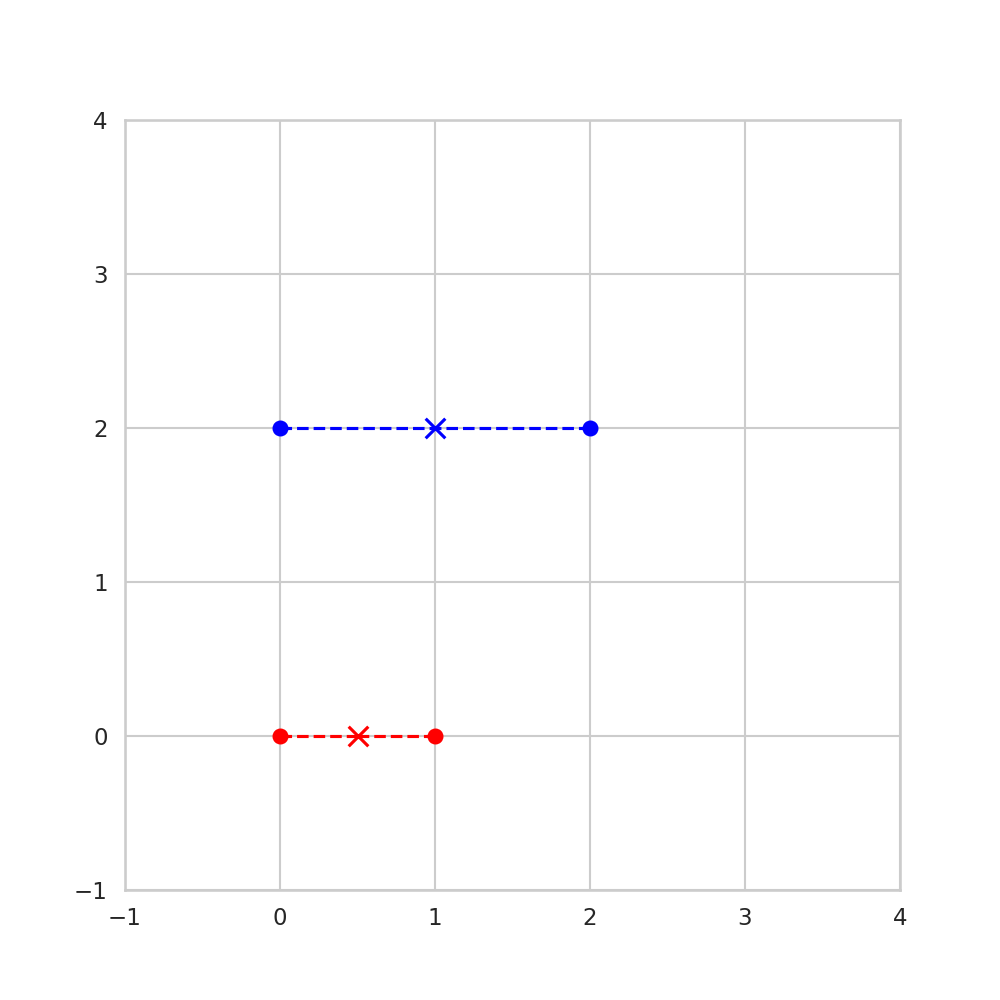
\includegraphics[width=0.43\textwidth]{assets/k-means-clusters.png}
    \label{fig:ex-1}
  \end{figure}

  Finally, regarding the \textbf{silhouette scores} of observations, we can compute them as follows
  (considering $s_n$ to be the silhouette of sample $x_n$ and $c_n$ to be its assigned cluster):

  \begin{equation*}
    \begin{aligned}
      s_n & = \frac{b_n - a_n}{\max\{a_n, b_n\}}                                                                            \\
      a_n & = \frac{1}{|c_n| - 1} \sum_{x_i \in c_n, x_i \neq x_n} \left\| x_i - x_n \right\|                               \\
      b_n & = \min_{n' \in \{1, \cdots, k\}, n' \neq n} \frac{1}{|c_{n'}|} \sum_{x_i \in c_{k'}} \left\| x_i - x_n \right\|
    \end{aligned}
  \end{equation*}

  Essentially, the silhouette score of a sample will take into account how close it is to
  the other samples in its cluster (in average), and how far it is from the samples in its
  most neighboring cluster (in average).

  \begin{equation*}
    \begin{aligned}
      a_1 & = \frac{1}{1} \left( \left\| x_2 - x_1 \right\| \right) =  1, \quad
      a_2 & = \frac{1}{1} \left( \left\| x_1 - x_2 \right\| \right) =  1        \\
      a_3 & = \frac{1}{1} \left( \left\| x_4 - x_3 \right\| \right) =  2, \quad
      a_4 & = \frac{1}{1} \left( \left\| x_3 - x_4 \right\| \right) = 2
    \end{aligned}
  \end{equation*}

  \begin{equation*}
    \begin{aligned}
      b_1 & = \min_{n' \in \{1, 2\}, n' \neq 1} \frac{1}{2} \left( \left\| x_3 - x_1 \right\| + \left\| x_4 - x_1 \right\| \right) = 2.414, \quad
      b_2 & = \min_{n' \in \{1, 2\}, n' \neq 1} \frac{1}{2} \left( \left\| x_3 - x_2 \right\| + \left\| x_4 - x_2 \right\| \right) = 2.236        \\
      b_3 & = \min_{n' \in \{1, 2\}, n' \neq 2} \frac{1}{2} \left( \left\| x_1 - x_3 \right\| + \left\| x_2 - x_3 \right\| \right) = 2.118, \quad
      b_4 & = \min_{n' \in \{1, 2\}, n' \neq 2} \frac{1}{2} \left( \left\| x_1 - x_4 \right\| + \left\| x_2 - x_4 \right\| \right) = 2.532
    \end{aligned}
  \end{equation*}

  \begin{equation*}
    \begin{aligned}
      s_1 & = \frac{2.414 - 1}{\max\{1, 2.414\}} = 0.5858, \quad
      s_2 & = \frac{2.236 - 1}{\max\{1, 2.236\}} = 0.5528        \\
      s_3 & = \frac{2.118 - 2}{\max\{2, 2.118\}} = 0.0557, \quad
      s_4 & = \frac{2.532 - 2}{\max\{2, 2.532\}} = 0.2102
    \end{aligned}
  \end{equation*}

  The silhouette scores for each cluster are given by the average of the silhouette
  scores of its samples:

  \begin{equation*}
    \begin{aligned}
      s_1 & = \frac{1}{2} \left( 0.5858 + 0.5528 \right) = 0.5693, \quad
      s_2 & = \frac{1}{2} \left( 0.0557 + 0.2102 \right) = 0.1329
    \end{aligned}
  \end{equation*}

  The overall silhouette score is given by the average of the silhouette scores of
  each cluster:

  \begin{equation*}
    s = \frac{1}{2} \left( 0.5693 + 0.1329 \right) = 0.3511
  \end{equation*}

  Finally, the \textbf{error classification rate} measures the proportion of misclassified
  samples in the dataset. If we think about the confusion matrix of the problem, we can
  write down the expression as:

  \begin{equation*}
    \begin{aligned}
      ECR & = \frac{FP + FN}{FP + FN + TP + TN} = \frac{(2 - 2) + (2 - 1)}{2 + 2} = 0.25
    \end{aligned}
  \end{equation*}

  \begin{tcolorbox}[enhanced jigsaw,halign=center,colback=bg,boxrule=0pt,arc=1pt]
    \item Consider the following unlabeled training data:

    \begin{table}[H]
      \centering
      \begin{tabular}{c|c|c|c}
              & $y_1$ & $y_2$ & $y_3$ \\ \hline
        $x_1$ & 1     & 0     & 0     \\
        $x_2$ & 8     & 8     & 4     \\
        $x_3$ & 3     & 3     & 0     \\
        $x_4$ & 0     & 0     & 1     \\
        $x_5$ & 0     & 1     & 0     \\
        $x_6$ & 3     & 2     & 1
      \end{tabular}
    \end{table}

    and let the initial $k$ centroids be the first $k$ samples.

    \begin{enumerate}
      \item Apply $k$-means until convergence, for $k \in \{2, 3\}$. What are the final centroids?
      \item Which $k$ provides a better clustering regarding \textbf{cohesion}
            (i.e the intra-cluster distance - the sum of the distances from every point to their centroid)?
      \item Which $k$ provides a better clustering regarding \textbf{separation}
            (i.e the inter-cluster distance - the average distance of every centroid to every other centroid)?
    \end{enumerate}
  \end{tcolorbox}

  Won't be doing the first question since it's basically repeating the last question's
  exercise (twice), and it's also in the teacher's solutions. We'll need the
  \textbf{post-convergence} centroids, though, so I'll write them down here (plus each
  cluster's assigned samples):

  \begin{paracol}{2}
    \setlength{\columnseprule}{1pt}
    \def\columnseprulecolor{\color{black}}
    \centering

    $k = 2$:

    \begin{equation*}
      \mu_1 = \begin{bmatrix}
  1.4\\
  1.2\\
  0.4\\
\end{bmatrix}, \quad \mu_2 = \begin{bmatrix}
  8\\
  8\\
  4\\
\end{bmatrix}
    \end{equation*}

    \begin{equation*}
      \begin{aligned}
        k_1 & = \{x_1, x_3, x_4, x_5, x_6\}, \quad
        k_2 & = \{x_2\}
      \end{aligned}
    \end{equation*}

    \switchcolumn

    $k = 3$:

    \begin{equation*}
      \mu_1 = \begin{bmatrix}
  0.333333\\
  0.333333\\
  0.333333\\
\end{bmatrix}, \quad \mu_2 = \begin{bmatrix}
  8\\
  8\\
  4\\
\end{bmatrix}, \quad \mu_3 = \begin{bmatrix}
  3\\
  2.5\\
  0.5\\
\end{bmatrix}
    \end{equation*}

    \begin{equation*}
      \begin{aligned}
        k_1 & = \{x_1, x_4, x_5\}, \quad
        k_2 & = \{x_2\}, \quad
        k_3 & = \{x_3, x_6\}
      \end{aligned}
    \end{equation*}

  \end{paracol}

  Regarding \textbf{cohesion}, we measure it as the sum of the distances from every
  point to their centroid. We can write down the expression as:

  \begin{equation*}
    \text{Cohesion}(k) = \sum_{i = 1}^k \sum_{x \in k_i} \left\| x - \mu_i \right\|^2
  \end{equation*}

  \begin{equation*}
    \begin{aligned}
      \text{Cohesion}(2) & = \left\| x_1 - \mu_1 \right\|^2 + \left\| x_2 - \mu_2 \right\|^2 + \left\| x_3 - \mu_1 \right\|^2 + \left\| x_4 - \mu_1 \right\|^2 + \left\| x_5 - \mu_1 \right\|^2 + \left\| x_6 - \mu_1 \right\|^2
                         &                                                                                                                                                                                                       & \approx 17.2 \\
      \text{Cohesion}(3) & = \left\| x_1 - \mu_1 \right\|^2 + \left\| x_2 - \mu_2 \right\|^2 + \left\| x_3 - \mu_3 \right\|^2 + \left\| x_4 - \mu_1 \right\|^2 + \left\| x_5 - \mu_1 \right\|^2 + \left\| x_6 - \mu_3 \right\|^2
                         &                                                                                                                                                                                                       & \approx 3.0
    \end{aligned}
  \end{equation*}

  Our goal is, ideally, to minimize this cohesion value: the closer the points are to
  their centroids, the better the clustering. We can see that $k = 3$ provides a
  better clustering in this regard, as expected: if there are more clusters, the
  points (generally speaking) should be able to better fit into them.

  \textbf{Separation}, on the other hand, is the average distance of every centroid to
  every other centroid. We can write down the expression as:

  \begin{equation*}
    \text{Separation}(k) = \frac{1}{k^2} \sum_{i = 1}^k \sum_{j = 1}^k \left\| \mu_i - \mu_j \right\|^2
  \end{equation*}

  \begin{equation*}
    \begin{aligned}
      \text{Separation}(2) & = \frac{1}{4} (\left\| \mu_1 - \mu_1 \right\|^2 + \left\| \mu_1 - \mu_2 \right\|^2 + \left\| \mu_2 - \mu_1 \right\|^2 + \left\| \mu_2 - \mu_2 \right\|^2)
      = \frac{1}{2} \left\| \mu_1 - \mu_2 \right\|^2
      \approx 51.38                                                                                                                                                                           \\
      \text{Separation}(3) & = \frac{1}{9} (\left\| \mu_1 - \mu_1 \right\|^2 + \left\| \mu_1 - \mu_2 \right\|^2 + \cdots \left\| \mu_3 - \mu_2 \right\|^2 + \left\| \mu_3 - \mu_3 \right\|^2)
      \approx 46.74
    \end{aligned}
  \end{equation*}

  As we've seen above, our previous goal was to minimize the cohesion value (for a
  better clustering solution); intuitively, we can say that growing separation values
  should lead to a better clustering solution, as well: the more separated the
  centroids are, (ideally) the better the clustering. We can see that $k = 3$ provides
  a worse clustering solution in this regard: the centroids are closer to each other,
  which means that the points could be more likely to be assigned to the wrong cluster.

  In the end, choosing the best $k$ value is a matter of balancing these (and other)
  metrics.

  \begin{tcolorbox}[enhanced jigsaw,halign=center,colback=bg,boxrule=0pt,arc=1pt]
    \item Consider the following data points:

    \begin{equation*}
      x_1 = (4), \quad x_2 = (0), \quad x_3 = (1)
    \end{equation*}

    Moreover, consider a mixture of two normal distributions with the following
    initialization of likelihoods and priors:

    \begin{equation*}
      \begin{aligned}
        \pi_1 & = P(c = k_1) = 0.5, \quad
              &                           & P(x | c = k_1) = \mathcal{N}(x; \mu_1, \sigma_1^2) = \mathcal{N}(x; 1, 1) \\
        \pi_2 & = P(c = k_2) = 0.5, \quad
              &                           & P(x | c = k_2) = \mathcal{N}(x; \mu_2, \sigma_2^2) = \mathcal{N}(x; 0, 1)
      \end{aligned}
    \end{equation*}

    Plot the clusters after a single iteration of the EM algorithm.

  \end{tcolorbox}

  The Expectation-Maximization (EM) algorithm is a powerful tool for cluster creation,
  learning the parameters of a distribution/mixture of distributions. It is a two-step iterative algorithm that
  alternates between two steps: the \textbf{Expectation} step and the
  \textbf{Maximization} step.

  Here, our centroids are precisely the means of each distribution; if in
  $k$-means we directly assigned the points to a cluster (and centroid updates
  would only take into account the samples assigned to them), in EM points aren't
  "assigned" to a given cluster, having rather a probability of belonging to each
  one of them. This way, parameter updates will always take into account
  \textbf{all} the points in the dataset (which should, ideally, lead us to a
  better clustering solution). This way, with each centroid being associated with
  a given distribution, we're not only able to know where the cluster's centroid
  is, but also its shape.

  In the \textbf{E-step}, we calculate the \textbf{posteriors} (i.e the probability/\textit{expectation}
  of a point belonging to each cluster), given the current parameters of the
  distributions. As we know, these probabilities can be written in function of the
  likelihoods and priors:

  \begin{equation*}
    \gamma_{ni} = P(c = k_i | x_n) = \frac{P(x_n | c = k_i) \pi_i}{\sum_{j = 1}^k P(x | c = k_j) \pi_j}
  \end{equation*}

  Since we know the priors in advance, we'll only need to calculate the likelihoods here.
  From the question's statement, we know that we can write down the likelihoods as:

  \begin{equation*}
    P(x | c = k_i) = \mathcal{N}(x; \mu_i, \sigma_i^2)
  \end{equation*}

  Computing this for each sample (and, for each one of them, for each cluster), we'll
  be able to gather the following (calculations will be shown in their entirety for the
  first sample, only final results for the remaining ones):

  \begin{equation*}
    \begin{aligned}
      \mathcal{N} (x_1; \mu_1, \sigma_1^2) & = \frac{1}{\sqrt{2 \pi \sigma_1^2}} \exp \left( - \frac{(x_1 - \mu_1)^2}{2 \sigma_1^2} \right) \\
                                           & = \frac{1}{\sqrt{2 \pi}} \exp \left( - \frac{(x_1 - 1)^2}{2} \right) = 0.004432                \\
      \mathcal{N} (x_1; \mu_2, \sigma_2^2) & = \frac{1}{\sqrt{2 \pi \sigma_2^2}} \exp \left( - \frac{(x_1 - \mu_2)^2}{2 \sigma_2^2} \right) \\
                                           & = \frac{1}{\sqrt{2 \pi}} \exp \left( - \frac{(x_1 - 0)^2}{2} \right) = 0.0001338
    \end{aligned}
  \end{equation*}

  \begin{equation*}
    \gamma_{11} = \frac{0.004432 \cdot 0.5}{0.004432 \cdot 0.5 + 0.0001338 \cdot 0.5} = 0.9707, \quad
    \gamma_{12} = \frac{0.0001338 \cdot 0.5}{0.004432 \cdot 0.5 + 0.0001338 \cdot 0.5} = 0.02931
  \end{equation*}

  Performing similar computations for the following samples, we're able to gather
  the following results:

  \begin{equation*}
    \begin{aligned}
      \mathcal{N} (x_2; \mu_1, \sigma_1^2) & = 0.242, \quad
      \mathcal{N} (x_2; \mu_2, \sigma_2^2) & = 0.3989, \quad
      \mathcal{N} (x_3; \mu_1, \sigma_1^2) & = 0.3989, \quad
      \mathcal{N} (x_3; \mu_2, \sigma_2^2) & = 0.242
    \end{aligned}
  \end{equation*}

  \begin{equation*}
    \begin{aligned}
      \gamma_{21} & = 0.3775, \quad
      \gamma_{22} = 0.6225, \quad
      \gamma_{31} & = 0.6225, \quad
      \gamma_{32} = 0.3775
    \end{aligned}
  \end{equation*}

  Having calculated the posteriors (and, subsequently, being able to perform an \textit{estimate
    of the probabilities of a sample belonging to each cluster}), we can move on to the
  \textbf{M-step}, where we'll update the parameters of the distributions, utilizing these
  new estimations. In this case, we'll be updating the means and std. deviations of each
  distribution, plus updating the priors afterward (note that when updating $\sigma$,
  we use the newly updated means).

  \begin{equation*}
    \mu_k = \frac{\sum_{n = 1}^N \gamma_{nk} x_n}{\sum_{n = 1}^N \gamma_{nk}}, \quad
    \sigma_k = \sqrt{\frac{\sum_{n = 1}^N \gamma_{nk} (x_n - \mu_k)^2}{\sum_{n = 1}^N \gamma_{nk}}}, \quad
    \pi_k = \frac{1}{N} \sum_{n = 1}^N \gamma_{nk}
  \end{equation*}

  \begin{paracol}{2}
    \setlength{\columnseprule}{1pt}
    \def\columnseprulecolor{\color{black}}
    \centering

    $k_1$:

    \begin{equation*}
      \begin{aligned}
        \mu_1    & = \frac{0.9707 \cdot 4 + 0 + 0.6225 \cdot 1}{0.9707 + 0.3775 + 0.6225} = 2.286 \\
        \sigma_1 & = 1.724,                                                                       \\
        \pi_1    & = 0.6569
      \end{aligned}
    \end{equation*}

    \switchcolumn

    $k_2$:

    \begin{equation*}
      \begin{aligned}
        \mu_2    & = \frac{0.02931 \cdot 4 + 0 + 0.3775 \cdot 1}{0.02931 + 0.6225 + 0.3775} = 0.4807 \\
        \sigma_2 & = 0.769,                                                                          \\
        \pi_2    & = 0.3431
      \end{aligned}
    \end{equation*}

  \end{paracol}

  After one EM epoch, we'll have the following:

  \begin{figure}[H]
    \centering
    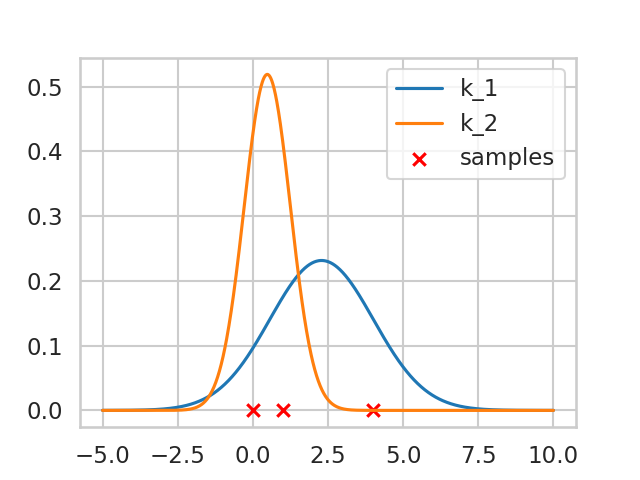
\includegraphics[width = 0.45\textwidth]{assets/ex-3-plot.png}
  \end{figure}

  \begin{tcolorbox}[enhanced jigsaw,halign=center,colback=bg,boxrule=0pt,arc=1pt]

    \textit{Note: even though the original question's statement doesn't mention the
      fact that the distributions are uniformly initialized, it's needed to solve
      this exercise.}

    \item Consider the following boolean data:

    \begin{table}[H]
      \centering
      \begin{tabular}{c|c|c|c|c}
              & $y_1$ & $y_2$ & $y_3$ & $y_4$ \\ \hline
        $x_1$ & 1     & 0     & 0     & 0     \\
        $x_2$ & 0     & 1     & 1     & 1     \\
        $x_3$ & 0     & 1     & 0     & 1     \\
        $x_4$ & 0     & 0     & 1     & 1     \\
        $x_5$ & 1     & 1     & 0     & 0     \\
      \end{tabular}
    \end{table}

    Assuming the presence of 3 clusters, variables to be conditionally independent, and
    the following priors:

    \begin{table}[H]
      \centering
      \begin{tabular}{c|c|c|c|c}
                & $P(y_1 = 1 \mid k = c)$ & $P(y_2 = 1 \mid k = c)$ & $P(y_3 = 1 \mid k = c)$ & $P(y_4 = 1 \mid k = c)$ \\ \hline
        $c = 1$ & 0.8                     & 0.5                     & 0.1                     & 0.1                     \\
        $c = 2$ & 0.1                     & 0.5                     & 0.4                     & 0.8                     \\
        $c = 3$ & 0.1                     & 0.1                     & 0.9                     & 0.2
      \end{tabular}
    \end{table}

    \begin{enumerate}
      \item Perform one EM iteration
      \item Verify that, after one iteration, the probability of the data increased
    \end{enumerate}

  \end{tcolorbox}

  Given that the distributions are uniformly initialized, we can assume that the
  priors are equal to $\frac{1}{K} = \frac{1}{3}$, with $K$ being the
  number of clusters of course.

  Moreover, given that all features all conditionally independent, all likelihoods
  can be computed as the product of the individual likelihoods:

  \begin{equation*}
    P(x_n \mid k = c) = \prod_{i = 1}^4 P(x_{ni} \mid k = c), \quad x_{ni} = x_n \text{'s } y_i
  \end{equation*}

  Let's perform the \textbf{E-step}. As usual, all steps are performed for the first sample
  (for both clusters), while for the remaining samples only the intermediate steps' results
  are shown.

  Regarding the first sample, we have the following likelihoods:

  \begin{equation*}
    \begin{aligned}
      P(x_1 \mid c = k_1) & = P(y_1 = 1 \mid c = k_1) \cdot P(y_2 = 0 \mid c = k_1) \cdot P(y_3 = 0 \mid c = k_1) \cdot P(y_4 = 0 \mid c = k_1) \\
                          & = 0.8 \cdot (1 - 0.5) \cdot (1 - 0.1) \cdot (1 - 0.1) = 0.324
    \end{aligned}
  \end{equation*}

  \begin{equation*}
    \begin{aligned}
      P(x_1 \mid c = k_2) & = P(y_1 = 1 \mid c = k_2) \cdot P(y_2 = 0 \mid c = k_2) \cdot P(y_3 = 0 \mid c = k_2) \cdot P(y_4 = 0 \mid c = k_2) \\
                          & = 0.1 \cdot (1 - 0.5) \cdot (1 - 0.4) \cdot (1 - 0.8) = 0.006
    \end{aligned}
  \end{equation*}

  \begin{equation*}
    \begin{aligned}
      P(x_1 \mid c = k_3) & = P(y_1 = 1 \mid c = k_3) \cdot P(y_2 = 0 \mid c = k_3) \cdot P(y_3 = 0 \mid c = k_3) \cdot P(y_4 = 0 \mid c = k_3) \\
                          & = 0.1 \cdot (1 - 0.1) \cdot (1 - 0.9) \cdot (1 - 0.2) = 0.0072
    \end{aligned}
  \end{equation*}

  Having gathered previously that all priors are equal to $\frac{1}{3}$, we can
  compute the (normalized) posterior probabilities as follows:

  \begin{equation*}
    \begin{aligned}
      \gamma_{11} & = \frac{P(x_1 \mid c = k_1) \cdot P(c = k_1)}{P(x_1)} = \frac{0.324 \cdot \nicefrac{1}{3}}{0.324 \cdot \nicefrac{1}{3} + 0.006 \cdot \nicefrac{1}{3} + 0.0072 \cdot \nicefrac{1}{3}} = 0.9609   \\
      \gamma_{12} & = \frac{P(x_1 \mid c = k_2) \cdot P(c = k_2)}{P(x_1)} = \frac{0.006 \cdot \nicefrac{1}{3}}{0.324 \cdot \nicefrac{1}{3} + 0.006 \cdot \nicefrac{1}{3} + 0.0072 \cdot \nicefrac{1}{3}} = 0.01779  \\
      \gamma_{13} & = \frac{P(x_1 \mid c = k_3) \cdot P(c = k_3)}{P(x_1)} = \frac{0.0072 \cdot \nicefrac{1}{3}}{0.324 \cdot \nicefrac{1}{3} + 0.006 \cdot \nicefrac{1}{3} + 0.0072 \cdot \nicefrac{1}{3}} = 0.02135
    \end{aligned}
  \end{equation*}

  Performing similar computations for the remaining samples, we obtain the following results:

  \begin{equation*}
    P(x_2 \mid c = k_1) = 0.001, \quad P(x_2 \mid c = k_2) = 0.144, \quad P(x_2 \mid c = k_3) = 0.0162
  \end{equation*}

  \begin{equation*}
    P(x_3 \mid c = k_1) = 0.009, \quad P(x_3 \mid c = k_2) = 0.216, \quad P(x_3 \mid c = k_3) = 0.0018
  \end{equation*}

  \begin{equation*}
    P(x_4 \mid c = k_1) = 0.001, \quad P(x_4 \mid c = k_2) = 0.144, \quad P(x_4 \mid c = k_3) = 0.1458
  \end{equation*}

  \begin{equation*}
    P(x_5 \mid c = k_1) = 0.324, \quad P(x_5 \mid c = k_2) = 0.006, \quad P(x_5 \mid c = k_3) = 0.0008
  \end{equation*}

  \begin{equation*}
    \begin{aligned}
       & \gamma_{21} = 0.006203, \quad &  & \gamma_{22} = 0.8933, \quad  &  &  & \gamma_{23} = 0.1005   \\
       & \gamma_{31} = 0.03968, \quad  &  & \gamma_{32} = 0.9524, \quad  &  &  & \gamma_{33} = 0.007937 \\
       & \gamma_{41} = 0.003439, \quad &  & \gamma_{42} = 0.4952, \quad  &  &  & \gamma_{43} = 0.5014   \\
       & \gamma_{51} = 0.9794, \quad   &  & \gamma_{52} = 0.01814, \quad &  &  & \gamma_{53} = 0.002418
    \end{aligned}
  \end{equation*}

  Regarding the \textbf{M-step}, we'll of course want to re-estimate the parameters
  according to the newly found posterior probabilities. In this case, however, we're no
  longer working with a Gaussian distribution representing the data; our parameters here
  will be the likelihoods and priors. The likelihoods, in particular, will be estimated
  using the following formula (considering that they're all conditionally independent):

  \begin{equation*}
    P(y_n \mid c = k_i) = \frac{\sum_{j=1}^N \gamma_{ji} x_{jn}}{\sum_{i=1}^N \gamma_{ji}}
  \end{equation*}

  The priors will be updated the same way as in the previous exercise.

  Regarding the first cluster, let's first compute each feature's prior likelihood:

  \begin{equation*}
    \begin{aligned}
      P(y_1 \mid c = k_1) & = \frac{\sum_{j=1}^N \gamma_{j1} x_{j1}}{\sum_{j=1}^N \gamma_{j1}}                                                                                         \\
                          & = \frac{0.9609 \cdot 1 + 0.006203 \cdot 0 + 0.03968 \cdot 0 + 0.003439 \cdot 0 + 0.9794 \cdot 1}{0.9609 + 0.006203 + 0.03968 + 0.003439 + 0.9794} = 0.9752
    \end{aligned}
  \end{equation*}

  \begin{equation*}
    P(y_2 \mid c = k_1) = 0.5153, \quad P(y_3 \mid c = k_1) = 0.0048, \quad P(y_4 \mid c = k_1) = 0.02479
  \end{equation*}

  The prior probability for this cluster will be computed as follows:

  \begin{equation*}
    P(c = k_1) = \frac{\sum_{j=1}^N \gamma_{j1}}{N} = \frac{0.9609 + 0.006203 + 0.03968 + 0.003439 + 0.9794}{5} = 0.3979
  \end{equation*}

  We're able to perform similar computations for the remaining clusters, gathering
  the following results:

  \begin{equation*}
    \begin{aligned}
       & P(y_1 \mid c = k_2) = 0.0151, \quad &  & P(y_2 \mid c = k_2) = 0.784, \quad P(y_3 \mid c = k_2) = 0.5842, \quad P(y_4 \mid c = k_2) = 0.9849 \\
       & P(y_1 \mid c = k_3) = 0.0375, \quad &  & P(y_2 \mid c = k_3) = 0.175, \quad P(y_3 \mid c = k_3) = 0.9500, \quad P(y_4 \mid c = k_3) = 0.9625
    \end{aligned}
  \end{equation*}

  \begin{equation*}
    P(c = k_2) = 0.4754, \quad P(c = k_3) = 0.1267
  \end{equation*}

  Regarding the second section of the exercise, we'll want to check whether, after
  an EM epoch, the \textbf{probability of the data increased} - that is, whether or not
  our distribution mixture is more likely to generate the data we're working with.
  Note that this is also a synonym of checking whether the \textbf{fitting probability} increasing.
  Considering conditionally independent variables, we're able to write this probability as
  the product of the probabilities of each sample:

  \begin{equation*}
    P(\mathbf{X}) = \prod_{n=1}^N P(\mathbf{x_n})
  \end{equation*}

  Moreover, we can also write the following:

  \begin{equation*}
    P(\mathbf{x_n}) = \sum_{i=1}^K \prod_{j=1}^M P(c = k_i) P(x_{nj} \mid c = k_i)
  \end{equation*}

  We have already calculated the likelihoods for each sample in the previous section;
  having done so, and since we also know the priors, we're able to easily
  compute $P(\mathbf{X})$ for before the EM epoch:

  \begin{equation*}
    P(\mathbf{X}) = \left(\frac{1}{3}\right)^5 (0.324 +  0.006 +  0.0072) \times \cdots \times (0.324 +  0.006 +  0.0008)
    = 4.88 \cdot 10^{-6}
  \end{equation*}

  Regarding the probability after the EM epoch, we'll need the feature-wise likelihood
  priors (which we have already calculated):

  \begin{equation*}
    \begin{aligned}
      P(\mathbf{X}) & = (0.3979 \cdot 0.9752 + 0.4754 \cdot 0.0151 + 0.1267 \cdot 0.0375) \times \cdots \times (\cdots + 0.1267 \cdot 0.9625) \\
                    & = 0.000186
    \end{aligned}
  \end{equation*}

  We can see that the probability of the data increased after the EM epoch: the mixture
  model has, then, become better at describing the data we're working with.

  \textit{Won't be doing the fifth question here since it's basically a copy of the
    third but with multivariate Gaussians, which are also covered in the fourth homework.}

  \begin{tcolorbox}[enhanced jigsaw,halign=center,colback=bg,boxrule=0pt,arc=1pt]

    \item Consider the following dataset (and an Euclidean distance space):

    \begin{table}[H]
      \centering
      \begin{tabular}{c|c|c}
              & $y_1$ & $y_2$ \\ \hline
        $x_1$ & 2     & 10    \\
        $x_2$ & 2     & 5     \\
        $x_3$ & 8     & 4     \\
        $x_4$ & 5     & 8     \\
        $x_5$ & 7     & 5     \\
        $x_6$ & 6     & 4     \\
        $x_7$ & 1     & 2     \\
        $x_8$ & 4     & 9     \\
      \end{tabular}
    \end{table}

    \begin{enumerate}
      \item Assuming observations $x_1$, $x_4$ and $x_7$ to be the initial seeds,
            identify the centroids after the first epoch using both $k$-means and $k$-medians.
      \item When is the median preferred over the mean?
    \end{enumerate}

  \end{tcolorbox}

  For starters, it's worth noting that, as expected, the variation between $k$-means
  and $k$-medians is exclusively related to the way the centroids are updated: instead
  of updating them utilizing the mean distance between each centroid and its assigned
  observations, $k$-medians will update them by taking the median distance between
  each centroid and its assigned observations - this way, the centroids shouldn't
  be affected by outliers as much as if they were updated using a mean.

  Let's start by assigning the samples to each cluster in the usual manner (note that, just as referenced
  in the question's statement, $k_1$ = $x_1$, $k_2$ = $x_4$ and $k_3$ = $x_7$, and that
  we're using the Euclidean distance):

  \begin{equation*}
    k_1 = \{x_1\}, \quad k_2 = \{x_3, x_4, x_5, x_6, x_8\}, \quad k_3 = \{x_2, x_7\}
  \end{equation*}

  We can now calculate the centroids for each cluster, using both $k$-means and $k$-medians.
  Regarding the former:

  \begin{equation*}
    \begin{aligned}
       & \bar{x}_1 = \frac{2}{1} = 2, \quad                 &  & \bar{y}_1 = \frac{10}{1} = 10               \\
       & \bar{x}_2 = \frac{8 + 5 + 7 + 6 + 4}{5} = 6, \quad &  & \bar{y}_2 = \frac{4 + 8 + 5 + 4 + 9}{5} = 6 \\
       & \bar{x}_3 = \frac{2 + 1}{2} = 1.5, \quad           &  & \bar{y}_3 = \frac{5 + 2}{2} = 3.5
    \end{aligned}
  \end{equation*}

  \begin{equation*}
    k_1' = \begin{pmatrix} 2 \\ 10 \end{pmatrix}, \quad
    k_2' = \begin{pmatrix} 6 \\ 6 \end{pmatrix}, \quad
    k_3' = \begin{pmatrix} 1.5 \\ 3.5 \end{pmatrix}
  \end{equation*}

  Regarding the latter:

  \begin{equation*}
    \begin{aligned}
       & m_x(1) = 2, \quad                                        &  & m_y(1) = 10                                       \\
       & m_x(2) = \operatorname{median}(8, 5, 7, 6, 4) = 6, \quad &  & m_y(2) = \operatorname{median}(4, 8, 5, 4, 9) = 5 \\
       & m_x(3) = \operatorname{median}(2, 1) = 1.5, \quad        &  & m_y(3) = \operatorname{median}(5, 2) = 3.5
    \end{aligned}
  \end{equation*}

  \begin{equation*}
    k_1'' = \begin{pmatrix} 2 \\ 10 \end{pmatrix}, \quad
    k_2'' = \begin{pmatrix} 6 \\ 5 \end{pmatrix}, \quad
    k_3'' = \begin{pmatrix} 1.5 \\ 3.5 \end{pmatrix}
  \end{equation*}

  (Note how the centroid remained the same, bar the $y$-coordinate of $k_2$'s centroid,
  which was updated from 6 to 5.)

  \begin{tcolorbox}[enhanced jigsaw,halign=center,colback=bg,boxrule=0pt,arc=1pt]

    Consider the following four scenarios of plotted data sets:

    \begin{figure}[H]
      \centering
      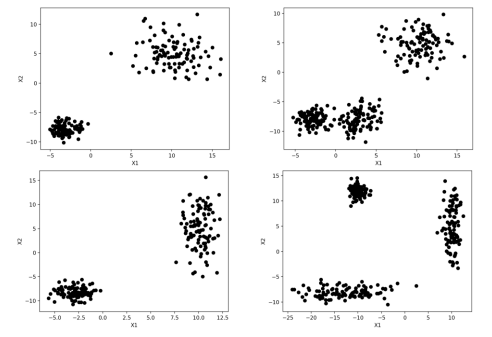
\includegraphics[width=0.4\textwidth]{assets/ex-9-plot.png}
    \end{figure}

    \begin{enumerate}
      \item For each scenario, justify whether $k$-means is suitable.
      \item Assuming EM clustering is applied to model all scenarios, what would
            the means and variances look like? For simplicity, assume that the covariance
            matrix is diagonal.
      \item When moving from numeric to ordinal data spaces, is the Hamming distance
            proper to handle ordinal data with high cardinality?
    \end{enumerate}

  \end{tcolorbox}

  As mentioned in this sheet's introduction, $k$-means is a clustering algorithm that
  creates circle/spherical-like clusters (while EM tends creates clusters shaped
  like its data's distributions). This way, if we have data where the clusters are
  not circular/spherical, $k$-means probably won't be the most suitable algorithm
  to use.

  \begin{enumerate}
    \item \textbf{Top-left}: we can clearly create a circle-like cluster for the
          bottom-left data points, while for the top-right ones, although not as clear,
          it does look like it's also possible to create a circle-like cluster for them;
          this way, we can say that $k$-means is suitable for this scenario (with $k=2$).
    \item \textbf{Top-right}: in the same manner as the previous scenario, we can
          create a circle-like cluster for the top-right data points; however, regarding
          the bottom-left data points, $k$-means will only be suitable if we're willing
          to split the points into left and right sections (otherwise we get an ellipse-like
          cluster). This way, $k$-means is only suitable here if we're working with $k=3$.
    \item \textbf{Bottom-left}: we can clearly create a circle-like cluster for the
          bottom-left data points, once again. However, there does not seem to be a way to
          avoid having an ellipse-like cluster for the right-most data points, hence
          $k$-means is not suitable for this scenario.
    \item \textbf{Bottom-right}: both the right-most and bottom-most data point clusters
          are clearly not circular/spherical, hence $k$-means is not suitable for this scenario.
  \end{enumerate}
\end{enumerate}

Regarding the second part of the question, the means will generally be wherever
the data's distributions are centered, while the covariance matrices will be
diagonal, with the diagonal values being the variances of each dimension - considering
ellipse-like clusters, for example, the variance will be obviously higher in the
"horizontal" (i.e the "first" in $\Sigma$) dimension, while it will be lower in the
"vertical" (i.e the "second" in $\Sigma$) dimension (vice-versa for vertically
elongated ellipses). Considering circle-like clusters, the variances will generally
be the same in both dimensions, with more spread out data points having higher
associated variances.

Finally, regarding whether the Hamming distance is suitable for ordinal data with
high cardinality, the answer is no. The Hamming distance is the most suitable
distance metric for data where there's no sense of "distance" between the values
of each dimension (e.g. the values of each dimension are just labels, like blood types).
Once we enter any type of data space where there's an intrinsic sense of "distance" between
the values of a given dimension, Hamming distance ends up being less and less suitable
for data with higher cardinality. Considering an example of ordinal data with low
cardinality, like "High", "Medium" and "Low", the Hamming distance between "High" and
"Medium" is 1, just like between "High" and "Low": while there should clearly be
a bigger difference between them (which would only be accentuated with higher and higher cardinality).

\end{document}